\title{Homework 1}
\author{
        Jerry Duncan
}
\date{\today}

\documentclass[12pt]{article}

\usepackage{amsmath}
\usepackage{graphicx}
\usepackage{pythonhighlight}


\begin{document}
\maketitle

\section{Problem 1}

\paragraph{Part a} The probability an egg breaks is given by $p$.
That means the probability an egg doesn't break is $1-p$.
Each egg's fate is determined independently so we can represent them as Bernoulli Random Variables where $P(break = success) = p$ and $P(intact = failure) = 1 - p$.
In that case, we can treat them collectively as a Binomial Random Variable since we desire to determine the number of successes out of L independent Bernoulli experiments.
$$P(x = 0\,\,break) = {L \choose 0}p^0(1-p)^{L-0} = (1-p)^L$$

\paragraph{Part b} For part b, we need to determine the chance that an egg breaks in one individual truck first.

$$P(x = 0) = {\frac{L}{N} \choose 0}p^0(1-p)^{\frac{L}{N}-0} = (1-p)^{\frac{L}{N}}$$

We then want to figure out what is the probability that that occurs for all $N$ trucks and since we are trying to find out the probability of two events happening independently but concurrently, we multiply $N$ times.

$$((1-p)^{\frac{L}{N}})^N = (1-p)^L$$

Which happens to be the same probability no eggs breaking when we transport all the eggs in one truck over $N$ trucks, so splitting up the shipment is neither harmful or helpful.

\section{Problem 2}

We are trying to find the probability that robot 1 is actually guarding the treasure given that he's told us "no". Specifically, then we are trying to find $P(guarding | no)$.
In the problem we are given a few more values, such as the probability robot 1 (or any of them for that matter) is guarding the treasure is $\frac{1}{3}$. That also means the probability a given robot is not guarding the treasure is $\frac{2}{3}$.
We are also given that $p_i$ is the probability that robot $i$ will tell us "no" when asked if he is guarding the treasure given that he actually is guarding it.
We have also been told that the probability a robot will say "no" when he is not guarding the treasure is $1$.
These values are summarized below.
\begin{gather*}
  P(r_i = guarding) = \frac{1}{3}        \\
  P(r_i = not\,\,guarding) = \frac{2}{3} \\
  P(r_i = no | guarding) = p_i           \\
  P(r_i = no | not\,\,guarding) = 1
\end{gather*}

So using Bayes Theorem we need to solve the following equation:
\begin{gather*}
  P(guarding | no) = \frac{P(no | guarding)P(guarding)}{P(no | guarding)P(guarding) + P(no | not\,\,guarding)P(not\,\,guarding)} \\
  P(guarding | no) = \frac{p_i * \frac{1}{3}}{p_i * \frac{1}{3} + 1 * \frac{2}{3}} = \frac{p_i}{p_i + 2}
\end{gather*}

After replacing $p_i$ with $p_1$ since we are looking at robot $1$, the answer is then $\frac{p_1}{p_1 + 2}$.

\section{Problem 3}

For this problem, we are given a few values.
Both players can be represented as their own Random Variables and due to the nature of how the problem is set up, they have similar symbolic representations, with only A or B replaced in their symbolic representations so I will only go through A's values for brevity.
\begin{gather*}
  P(shot) = p_A            \\
  P(no\,\,shot) = 1 - p_A  \\
  P(miss | shot) = m_A     \\
  P(make | shot) = 1 - m_A \\
  P(shot | miss) = 1       \\
  P(shot | make) = 1
\end{gather*}

\paragraph{Part a}
For part a, we want to figure out the mean of T, a Random Variable that represents the number of shots made in a given time period. Because it is a summation of the Random Variables representing the number of shots A and B make, we can then add their individual expected values to arrive at the answer. In order to answer this, we need to calculate the probability that A and B either make their shot or miss it.

\begin{gather*}
  P(miss) = \frac{P(miss | shot)P(shot)}{P(shot | miss)} = \frac{m_A * p_A}{1} = m_A * p_A \\
  P(make) = \frac{P(make | shot)P(shot)}{P(shot | make)} = \frac{(1 - m_A)(p_A)}{1} = (1 - m_A)p_A
\end{gather*}

Now with these values, we can calculate the expected values of A and B. Remember that anywhere there is a $X_A$, we can put $X_B$ and the formulas stay the same.

\begin{gather*}
  E[T] = E[A] + E[B]                                                            \\
  E[A] = 0 * (P(miss) + P(no\,\,shot)) + 1 * (P(make)) = P(make) = (1 - m_A)p_A \\
  E[B] = 0 * (P(miss) + P(no\,\,shot)) + 1 * (P(make)) = P(make) = (1 - m_B)p_B
\end{gather*}

So the answer for part a is $E[T] = (1 - m_A)p_A + (1 - m_B)p_B$

\paragraph{Part b} For part b, we're asked to calculate the probability that at least one shot is made during a time slot, but that is complicated. Instead, we can subtract the probability of 0 shots made from 1. To find the probability that each makes no shots, we can do a similar substitution and subtract the probability of making a shot from 1.

\begin{gather*}
  P(make) = (1 - m_A)p_A                                             \\
  P(not\,\,making) = 1 - (1 - m_A)p_A                                \\
  P(both\,\,don't\,\,make) = (1 - (1 - m_A)p_A) * (1 - (1 - m_B)p_B) \\
  P(at\,\,least\,\,one\,\,make) = 1 - (1 - (1 - m_A)p_A) * (1 - (1 - m_B)p_B)
\end{gather*}

So the answer to part b is $P(at\,\,least\,\,one\,\,make) = 1 - (1 - (1 - m_A)p_A) * (1 - (1 - m_B)p_B)$.

\paragraph{Part c} For part c, we can use the value we calculated for $P(both\,\,don't\,\,make)$ and extend it to $N$ time slots. All we need to do is multiply it $N$ times.

So the answer to part c is $((1 - (1 - m_A)p_A) * (1 - (1 - m_B)p_B))^N$.


\section{Problem 4}

\paragraph{Part a} For part a, we're taking a look at the softmax formula in a Reinforcement Learning context. The formula for that is below.

\begin{gather*}
  P(A_t = a) = \frac{e^{\frac{H_t(a)}{\tau}}}{\sum_{b=1}^n e^{\frac{H_t(b)}{\tau}}}
\end{gather*}

If we replace $H_t(a)$ with the average reward of the $n$-armed bandit, we end up with the following:
\begin{gather*}
  P(A_t = a) = \frac{e^{Q_t(a)}}{\sum_{b=1}^n e^{Q_t(b)}}
\end{gather*}

Because each of the arms are independent and identically distributed, $Q_t(a) = Q_t(b) \forall b \in n$. And $Q_t(a) = \frac{1}{p} \forall a \in n$. The mean of a geometric distribution is $\frac{1}{p}$ and each arm has the same $p$ due to being i.i.d. This reduces the softmax equation further to:
\begin{gather*}
  P(A_t = a) = \frac{e^{\frac{1}{p}}}{\sum_{b=1}^n e^{\frac{1}{p}}}
\end{gather*}

This causes each arm to have an equal chance, $\frac{1}{n}$, of being selected by our softmax policy.

\paragraph{Part b} For part b, we want to calculate the expected reward per turn using that policy. Because that policy results in each arm being picked equally likely, we need to find the expected reward given a random arm. And because each arm is i.i.d., each has the same expected reward, $\frac{1}{p}$.

\paragraph{Part c} For part c, we need to determine if an $\epsilon$-greedy approach would change the average reward. The answer is it would not because all arms have an equal expected reward so there is no difference between picking each arm with a random change (softmax policy) and picking the best arm (which is a $n$-way tie) 1-$\epsilon$\% of the time and a random arm $\epsilon$\% of the time. To be clear, no, it doesn't change the answers to part a or part b.

\section{Problem 5}

In Table \ref{tab:problem-5}, I've included the full table for calculating estimated reward and average reward per turn. To make it excessively clear, this table is laid out slightly different than the example in class. At each time step t, all values are calculated based on $A_t$ being taken and $R_t$ being given. That means that at step 0, all Q values are the initial estimates and at step 1, Q(1) has already been updated to reflect $R_1$.

\paragraph{Part a} For part a, we need to determine which time steps the $\epsilon$ case occurred.
That is that we took an action that was \textit{clearly} not the best.
In this case, at step 3, 5, and 6, we took actions that went against what the best estimated reward suggested.
At step 3 we chose action 3 despite action 2 being the clear best at the time.
At step 5 we took action 3 despite action 2 still being the best.
And at step 6 we took action 4, despite action 2 being the best.

\paragraph{Part b} For part b, we need to determine which time steps that the $\epsilon$ \textit{could} have occurred, but not definitively.

Since we know nothing about how the agent breaks ties, step 1 and step 2 are both times where we \textit{could} have taken the $\epsilon$ case, but there is no way to tell for sure.
At step 1 we chose action 1, despite them all being tied.
And at step 2, we chose action 2, despite 4 of them still being tied for highest.

\paragraph{Part c} For part c, we need to calculate the average reward the agent received after every step. While this is included in the last column of Table \ref{tab:problem-5}, I've included it in Table \ref{tab:problem-5-avg} as well. To be clear the tables show the reward per turn \textit{after} $A_t$ has been taken and $R_t$ was given.

\begin{table}[!htb]
  \centering
  \label{tab:problem-5-avg}
  \begin{tabular}{|c|c|c|c|c|c|c|c|}
    \hline
    Step        & 0 & 1  & 2   & 3 & 4   & 5   & 6                 \\
    \hline
    Avg. Reward & 0 & -2 & 0.5 & 0 & 0.5 & 0.4 & $1.1\overline{6}$ \\
    \hline
  \end{tabular}
\end{table}


\begin{table}[!htb]
  \centering
  \label{tab:problem-5}
  \begin{tabular}{|c|c|c|ccccc|c|}
    \hline
    Step & $A_t$ & $R_t$ & Q(1) & Q(2)            & Q(3)           & Q(4) & Q(5) & Avg Reward / Turn \\ \hline
    0    & -     & -     & 0    & 0               & 0              & 0    & 0    & 0                 \\ \hline
    1    & 1     & -2    & -2   & 0               & 0              & 0    & 0    & -2                \\ \hline
    2    & 2     & 3     & -2   & 3               & 0              & 0    & 0    & 0.5               \\ \hline
    3    & 3     & -1    & -2   & 3               & -1             & 0    & 0    & 0                 \\ \hline
    4    & 2     & 2     & -2   & 2 $\frac{1}{2}$ & -1             & 0    & 0    & 0.5               \\ \hline
    5    & 3     & 0     & -2   & 2 $\frac{1}{2}$ & -$\frac{1}{2}$ & 0    & 0    & 0.4               \\ \hline
    6    & 4     & 5     & -2   & 2 $\frac{1}{2}$ & -$\frac{1}{2}$ & 5    & 0    & $1.1\overline{6}$ \\ \hline
  \end{tabular}
\end{table}

\section{Problem 6}

\paragraph{Part a} For part a I've included the output and the code used to generate that output. This doesn't include the graphing code in part b.

\inputpython{problem_6.py}{1}{20}

\begin{python}
  '''
  Problem 6 Output
  '''
  Alpha: 0.5, Series 1, Last Update: 1.998046875
  Alpha: 0.25, Series 1, Last Update: 1.8873729705810547
  Alpha: 1, Series 1, Last Update: 2
  Alpha: 0.5, Series 2, Last Update: 3.935546875
  Alpha: 0.25, Series 2, Last Update: 3.4127635955810547
  Alpha: 1, Series 2, Last Update: 4
  Alpha: 0.5, Series 3, Last Update: 3.330078125
  Alpha: 0.25, Series 3, Last Update: 2.965871810913086
  Alpha: 1, Series 3, Last Update: 4
  Alpha: 0.5, Series 4, Last Update: 2.05859375
  Alpha: 0.25, Series 4, Last Update: 2.2493553161621094
  Alpha: 1, Series 4, Last Update: 2
\end{python}

\paragraph{Part b} For part b, I've included Figure \ref{fig:series-1}, \ref{fig:series-2}, \ref{fig:series-3}, and \ref{fig:series-4} that show the average rewards for each alpha across the three series we've been asked about as well as another series that mimics an inverse step-down function for its reward.

For the constant reward of Series 1, and likely for any constant reward, the larger the alpha is, the faster our estimate of $q_*(a)$ equals its real value.

For the step-style rewards of Series 2 and Series 4, a larger alpha seems to help get to $q_*(a)$ faster than a small one, similar to the constant reward distributions. It's possible that when the reward changes at a different point than the midpoint that that is not the case. And even in the case where it does change in the middle of the series, I think a small epsilon is still a reasonable choice.

Lastly, for the randomly changing rewards of Series 3, a smaller epsilon is best. While it does take a little longer to reach a $Q(a)$ that is close to $q_*(a)$, it provides an estimate that is closest to the actual average.



\begin{figure}
  \centering
  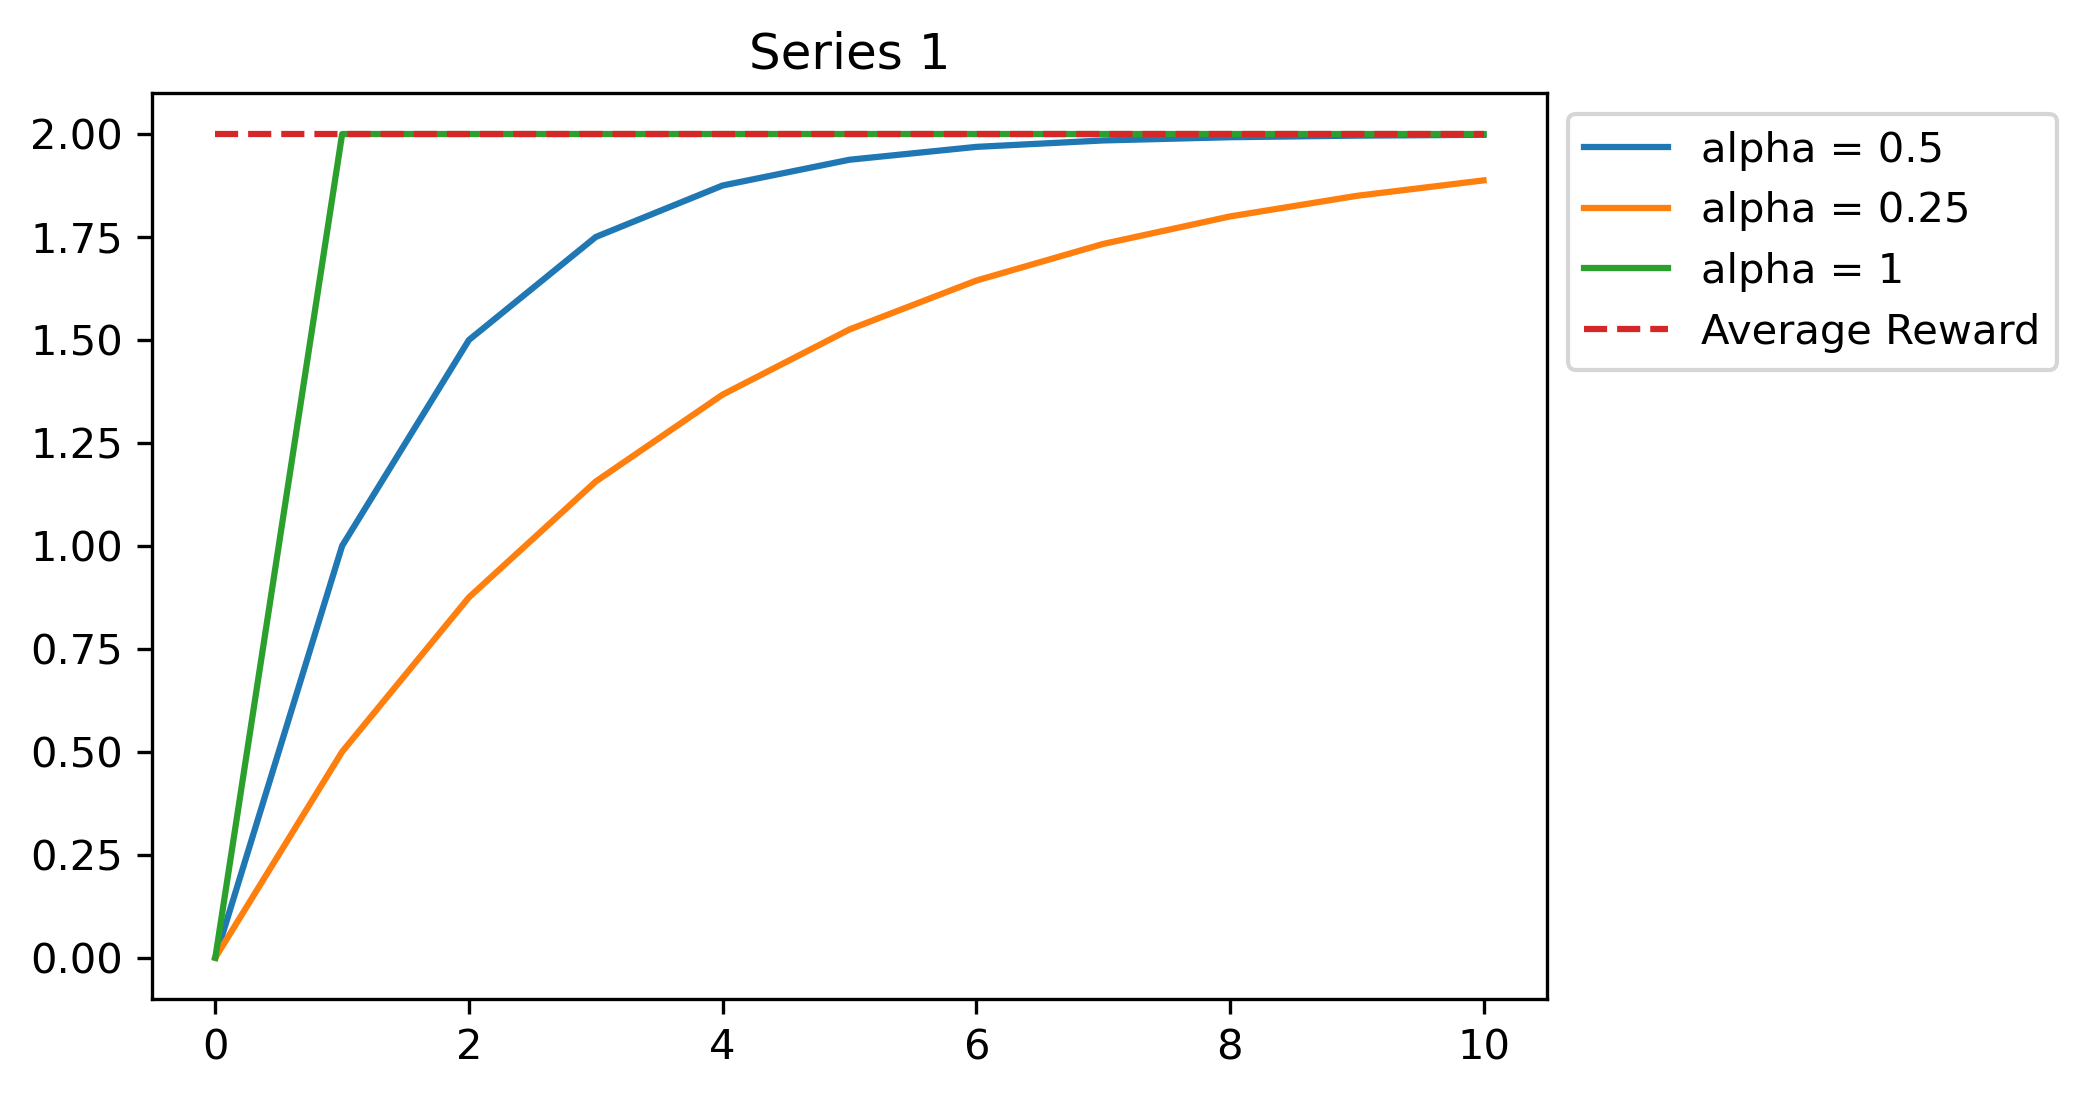
\includegraphics[width=\linewidth]{series_1.png}
  \caption{Series 1 vs Alpha}
  \label{fig:series-1}
\end{figure}

\begin{figure}
  \centering
  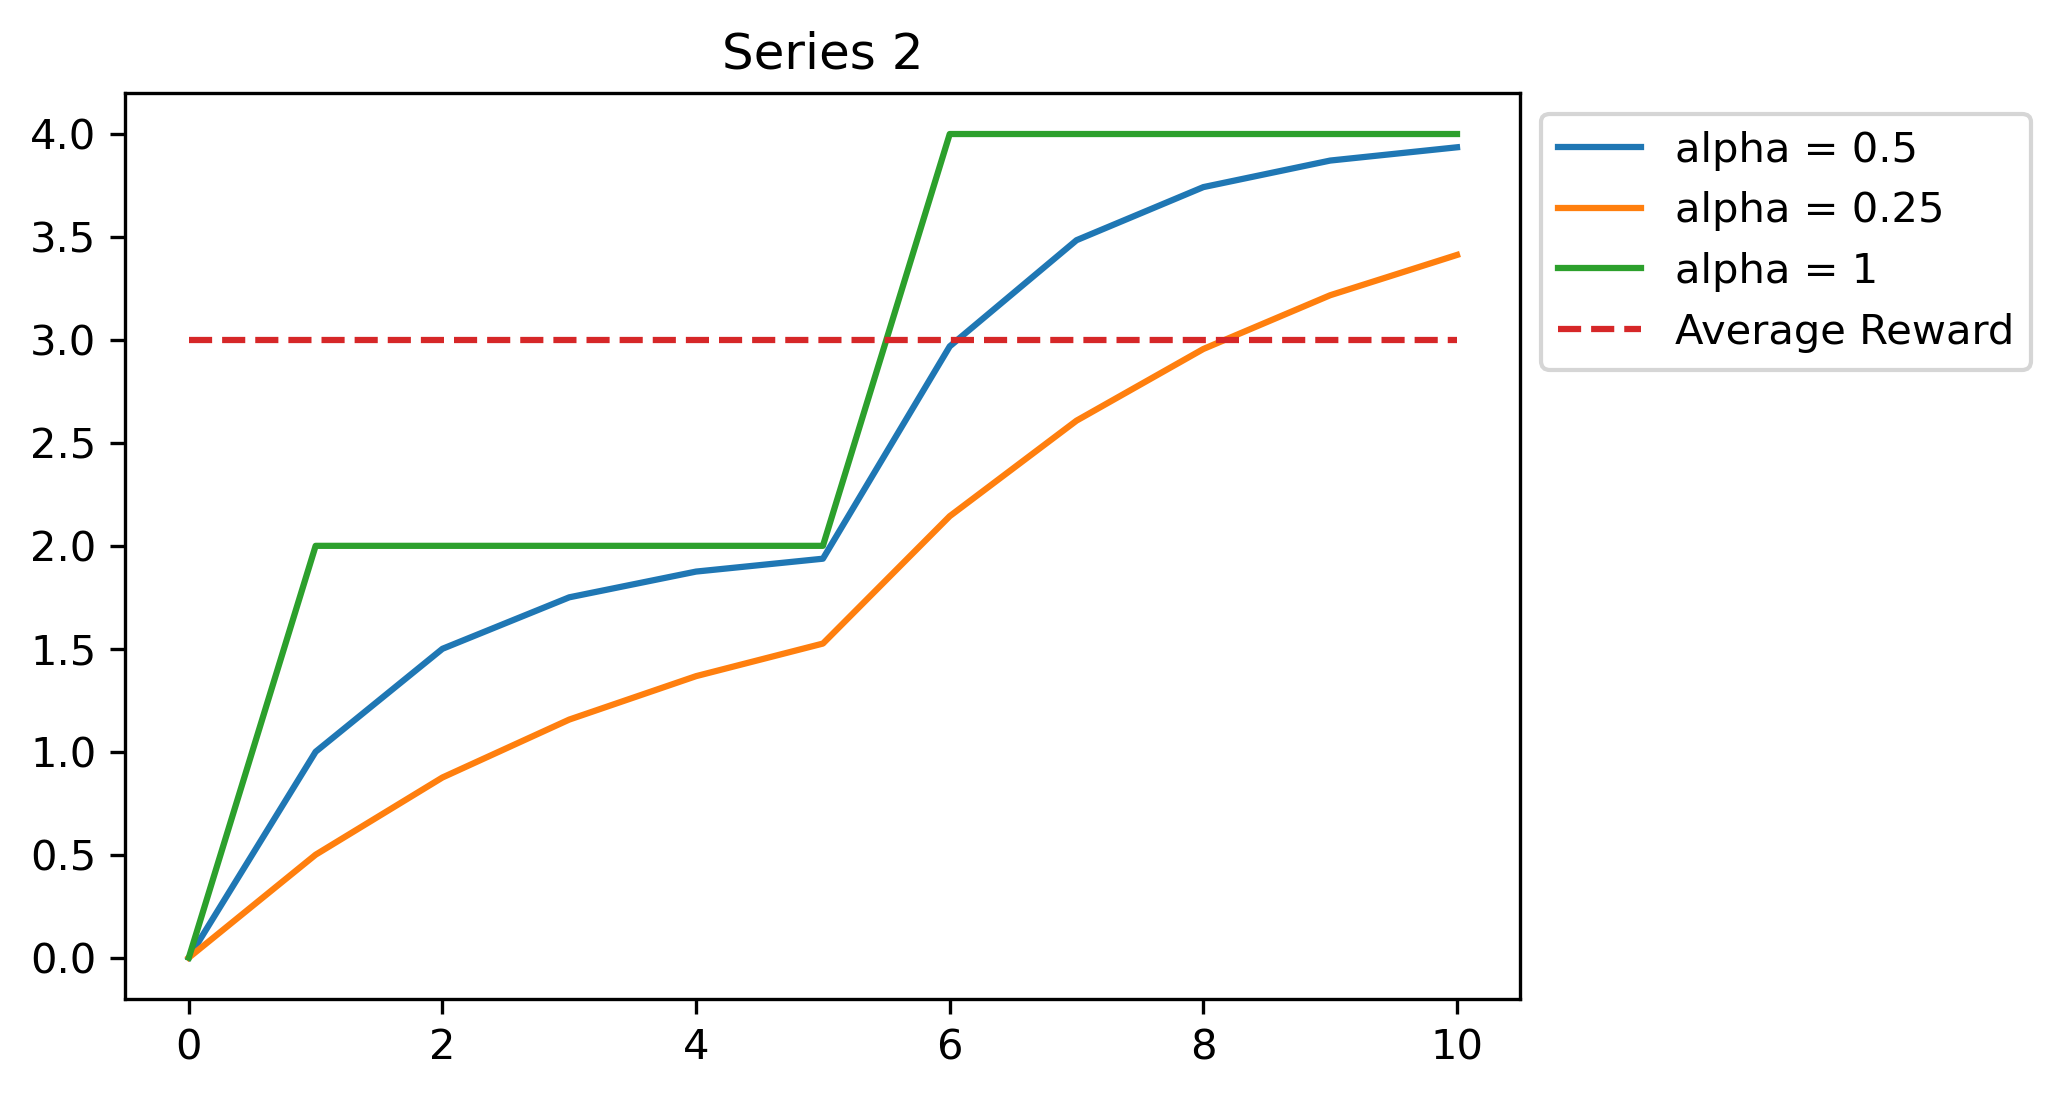
\includegraphics[width=\linewidth]{series_2.png}
  \caption{Series 2 vs Alpha}
  \label{fig:series-2}
\end{figure}

\begin{figure}
  \centering
  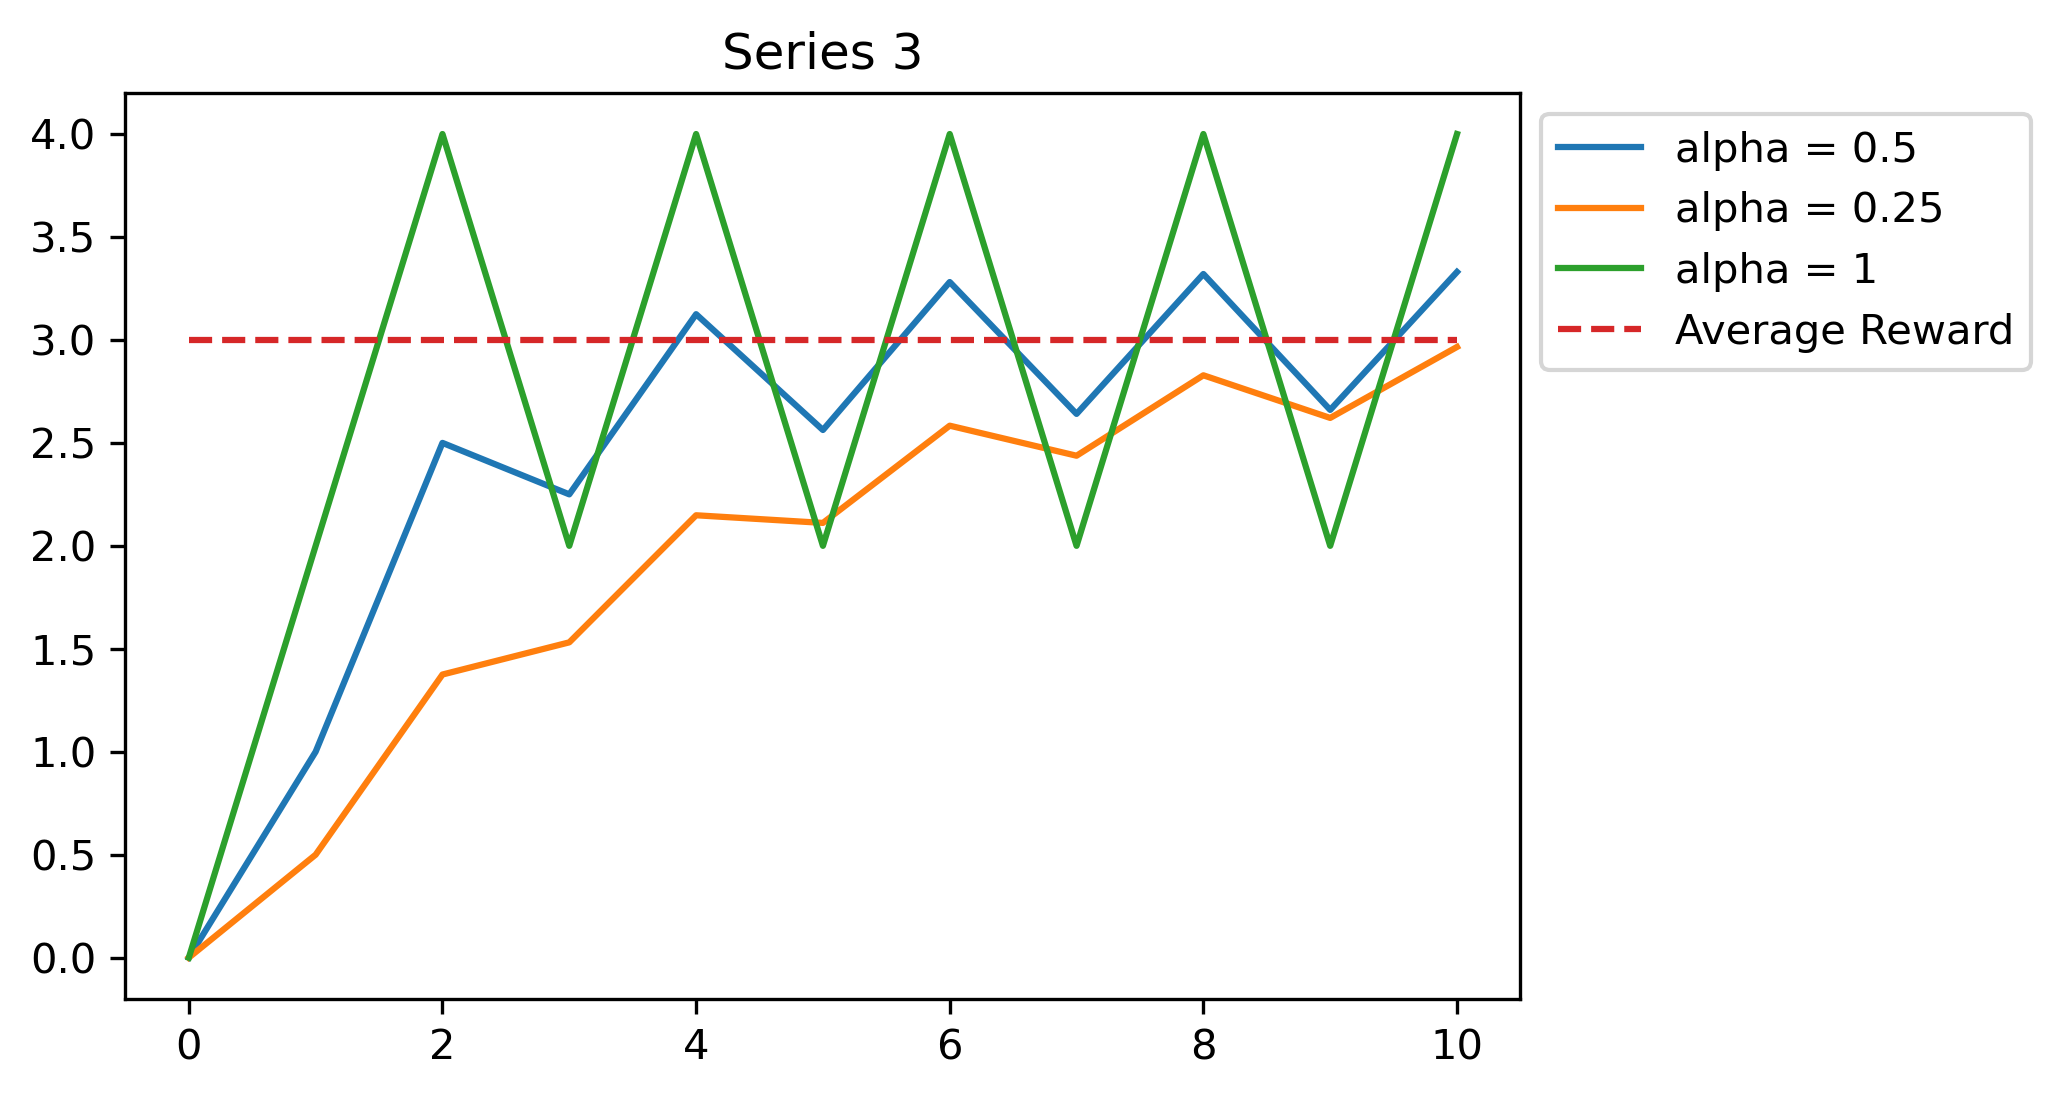
\includegraphics[width=\linewidth]{series_3.png}
  \caption{Series 3 vs Alpha}
  \label{fig:series-3}
\end{figure}

\begin{figure}
  \centering
  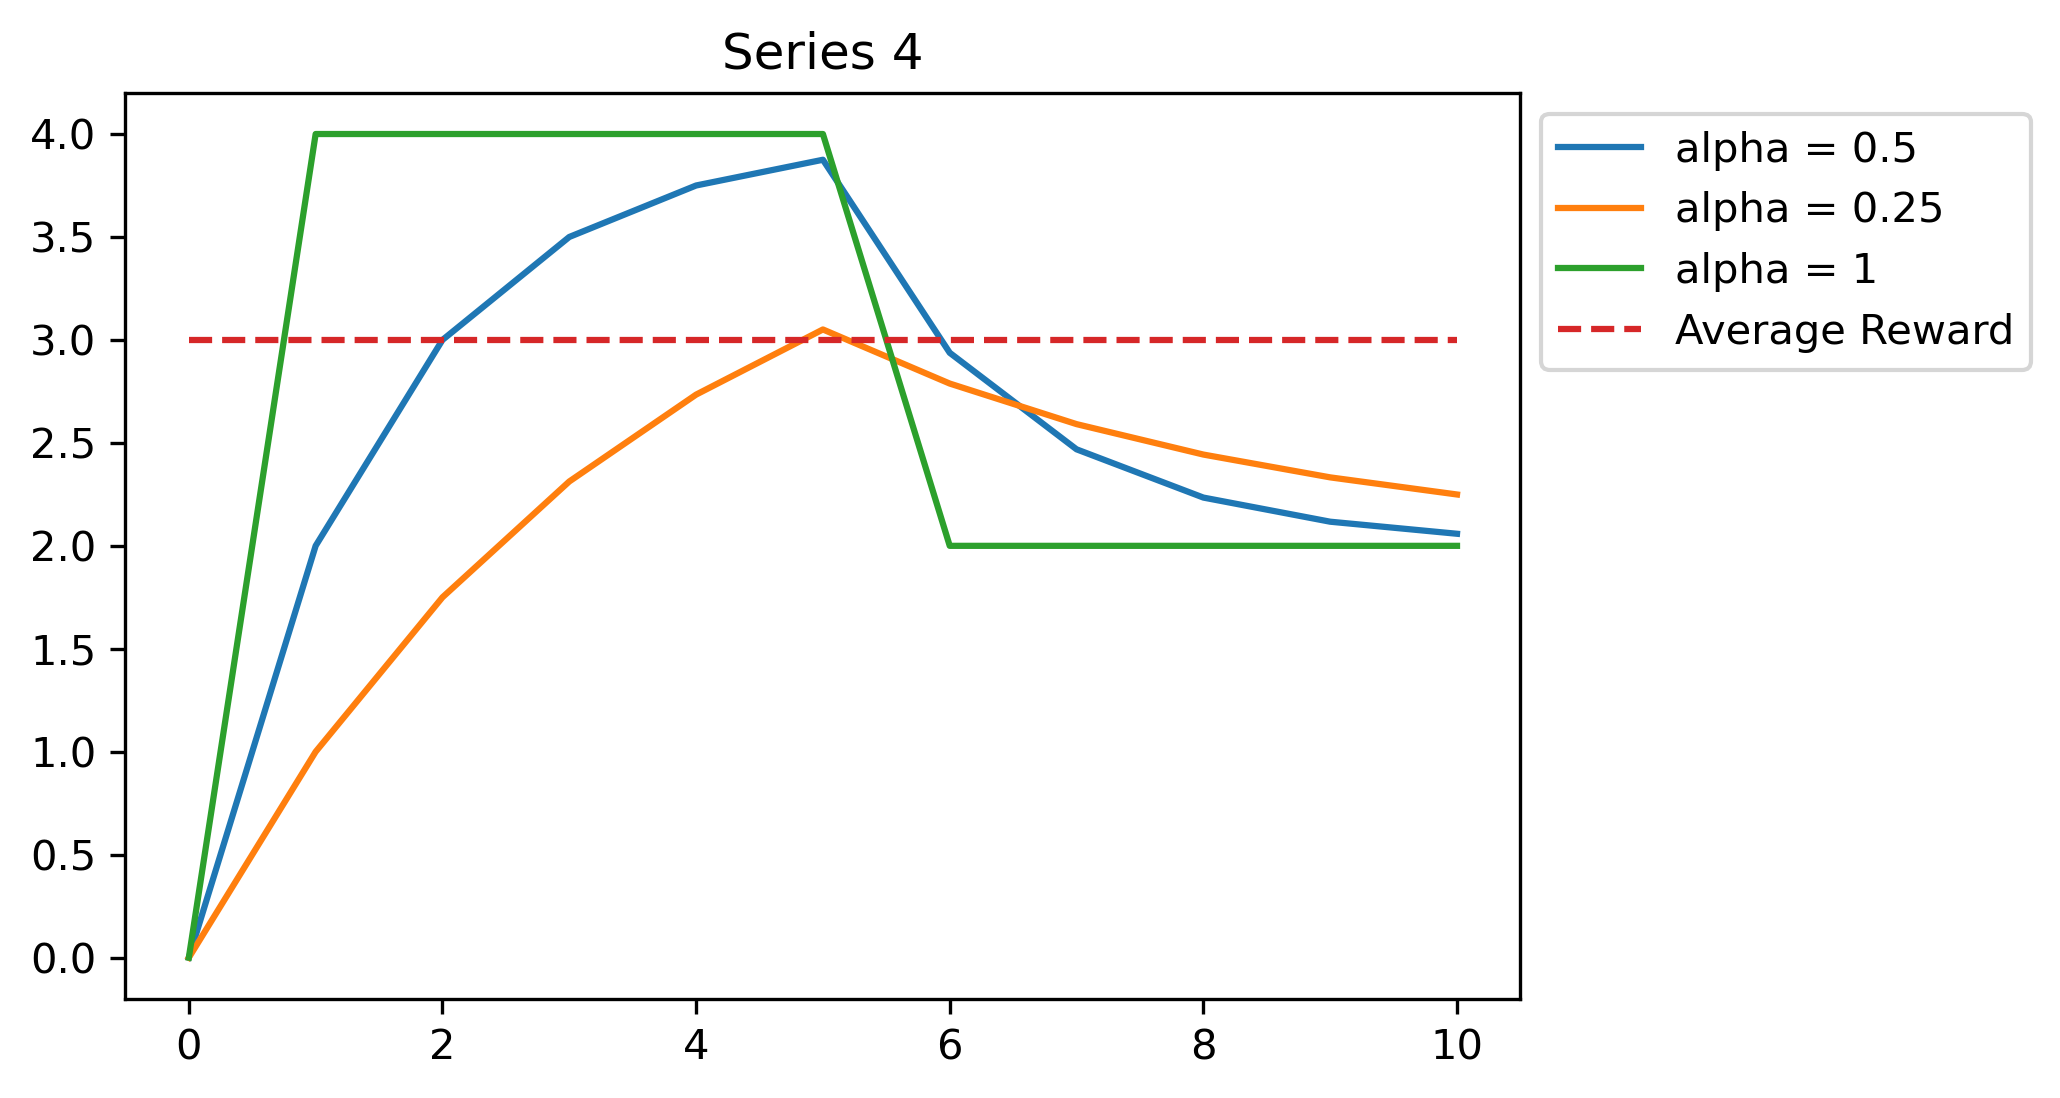
\includegraphics[width=\linewidth]{series_4.png}
  \caption{Series 4 vs Alpha}
  \label{fig:series-4}
\end{figure}

\bibliographystyle{abbrv}
\bibliography{main}

\end{document}